\documentclass{standalone}
% preamble: usepackage, etc.
\begin{document}

\chapter{相关技术和理论}
人工智能的发展走过了从机器智能到感知智能的阶段,正在迈向认知智能的阶段。
但要实现认知智能,机器必须学会处理人类复杂的语言,学会做知识的推理,这是
人工智能遇到的一大难题。目前通过机器的深度学习和知识图谱推理相结合,能够
很好的解决人类自然语言的语义鸿沟。
\section{知识图谱}
知识图谱是一种规模非常大的语义网络系统,它主要目的就是为了描述真实世界
里实体或者概念的关联关系。通过大量数据手机,整理成机器能处理的知识库,
实现可视化的展示。

目前知识库的构建主要有两个种类:一类是Curated KBs,主要是通过结构化
的构建,优点在于结构简单,脏数据比较少,目前是行业内使用比较多的构建
方法,如维基百科;一类是Extracted KBs,这是一种三元组结构,抽取的实体
多样性,实体关系更多的是自然语言的形式。
\subsection{知识图谱概述}
近些年,对知识图谱的研究越来越受关注,越来越火热,知识图谱有着各种各样的
定义,再知识图谱发展的各个时期的定义和特点都是不一样的,早在计量学以及
科学计量时期就已经开始有对知识图谱的研究了【30】。这个时期的知识图谱
主要的形式是一些比较简单的二维图形,也有三维图,主要是用来表示科学方面
的统计结果;“三维构型图谱”是由著名的计量学家格蕾汽摩在1987年的时候
创立的【31】,而之后又出现了“多维知识图谱“。在2012年谷歌提出知识图谱并
将去用于语义搜索之后,知识图谱再一次涌入学者的研究视线,将这些蕴含着人类
大量先验知识的知识图谱与深度学习融合成为了进一步提升人工智能效果重要
思路之一,知识图谱的地位也再一次得到了重视。知识图谱在问答领域同样
发挥着知识承载的作用,问答系统是搜索系统的进阶交互形式,为了能让对话
系统更加准确和可靠的给出想要的信息,其背后一定要依托一个巨大的知识图谱。
比如熟悉的苹果手机的智能语音助手Siri就依托于一Wolffram Alpha公司为提供
的知识搜索技术。此外,通过构建各个领域,例如,金融、医药、电商、企业、教育
等的知识图谱,可以帮组金融从业者、医患人员、买卖卖家等对待问题进行辅助
决策。利用知识图谱与深度学习进行一些常识的推理等工作也是目前众多学者
正在研究和攻克的方向。

知识图谱可以最有效、最直观地表达出实体间的关系。简单地说,就是把大量不同
种类的信息连接在一起而得到一个关系网络,为人们提供了从“关系”的角度分析
问题的能力。相对于传统的描述方式,知识图谱具有一些自身的特点:实体的识别
是从文本中抽取特定的实体信息,这是依赖于自然语言中的命名体识别技术,这些
实体构成了知识图谱中的点。关系的识别是指实体间的各种关系,这些关系确定了
知识图谱点与点之间的边。需要说明的是,常用抽取关系的方法有基于专家知识库
和基于机器学习等类型。其中,基于专家知识库的方法是由行业专家构筑大规模的
领域知识库,需要专业领域的人参与构建,较为耗时费力。但是质量相对比较可靠;
机器学习的方法需要构造特征向量形式的训练数据,使用机器学习算法自动构造。
需要特别指出的是,对于非结构化文本,实体类别和关系抽取需要基于自然语言
处理算法,以及深度学习算法(例如,用词向量的方式寻找近义词,提高实体
模糊识别的准确率),这是一个反复迭代、不断精进的过程。

知识图谱的引入使得传统的基于网页的搜索方式得到了补充,让搜索直指答案
本身,也就是说从传统的链接文本转为链接数据,即Web of Texts,Web of
Documents到Web of Data,Web of Objects的转变,这种方式能让我们将
复杂的不便与计算机分析处理的文本数据转换为基于实体的、对象的数据,
使得计算机能更好地建立实体之间的连接关系。
\subsubsection{语义网络与语义网}
Quilian在1968年提出的知识表达模式,其用相互连接的节点和边表示知识。
完全由用户自定义,无任何标准和规范,难以用于实践。
*************语义网络图2-1
而语义网是Tim.Lee在1998年提出的一个新概念,描述互联网中资源和数据
之间的关系,使得互联网上的数据变得机器可读。常被用来指代一套完整技术
栈框架。即,语义网比语义网络更高级的概念,它提供了一整套规范和技术栈
来解决实际问题。
\subsubsection{语义网的技术栈}
下图2-2是行业知识图谱主要技术标准
*****************
1)编码方式(UNICODE),资源标识符(URI):数据的编码方式和表示方式
2)数据序列化方法(Syntax):数据的序列化方法,包括不仅限于XML,N-Triples,
Turtle,Json-LD 
3)数据描述框架(RDF):数据模型,表示知识的一种方法和手段
4)RDFs/OWL:工业标准,使用预定义的词汇,对RDF进行类和属性定义,即,
Schema。用概念(Class),对象属性(Object Property)和数据属性
(Data Property)分别表示实体,关系和数据
5)RIF/SWRL:推理规则(Rule),使用预定义的规范,使基于RGFs和OWL
描述的RDF数据具有推理能力
6)SPARSQL:基于RDF+(RDFs/OWL:optional)的查询语言
7)其他:Cryptograpgy+Logic+Proof+Trust:中间层概念,决定应用层
如何确定数据可靠,精确和值得信赖
\section{产生式系统}
产生式系统是给定事实与推理规则,进行自动推理的推理系统。产生式系统
是由3个部分组成:总数据库、产生式规则、控制策略。总数据库是存放求解
过程中各种当前信息的数据结构,包括已知事实与推理过程中得到的结论;
产生式郭泽是一个规则库,存放形如“if <前提>, then <结论>" 的推理
规则;控制策略决定了推理过程中如何应用规则,即确定下一步应该选
用什么规则以及进行适当的冲突消解,类比于图搜索中的图搜索策略
(DFS,BFS,etc.)。下图2-2是产生式系统与图搜索
*******************

按照搜索方向,产生式系统可分为正向推理、逆向推理和双向推理。
例 正向推理 设P1,P2,P3,P4 为谓词公式或命题, 初始总数据库 DB={P1},
 规则库 R={R1:P1→P2,R2:P2→P3,R3:P3→P4}, 则推理步骤如下
P1∈DB, 在规则库R中寻找到可用的规则 R1:P1→P2, 得到 P2, 当前DB={P1,P2}
P2∈DB, 在规则库R中寻找到可用的规则 R2:P2→P3, 得到 P3, 当前DB={P1,P2,P3}
P3∈DB, 在规则库R中寻找到可用的规则 R3:P3→P4, 得到 P4, 当前DB={P1,P2,P3,P4}

其中控制系统常用控制策略以及常用算法包括:
(1)正向推理算法主要处理步骤:
**********************
(2)逆向推理:
*********************

产生式表示法的特点也十分明显,采用”如果xxx则xxx“的形式表示知识,
非常直观自然,便于推理。同时规则库、数据库和控制系统策略完全分离,
三者相互独立,居于良好的可扩展性并且模块化程度高。规则格式简单、
固定,仅由条件和结论(或操作)组成。但是产生式系统也有先天的局限性:
效率不是很高,推理求解过程一般都有匹配、执行和冲入消解三个步骤。
并且在数据库和规则库十分庞大的情况下,容易引起知识的组合爆炸。
而且在规则库和数据库十分庞大时,对规则的描述必须十分谨慎,对应
这产生式规则的条件部分描述会变得特别复杂,会导致匹配的复杂度增加,
使得匹配效率急剧下降。另外,每条规则对应一个独立的程序单元,相互
之间的调用会比较困难,因此不太适合复杂理论要求的问题。
\section{图数据库Neo4j}
\subsection{图数据库概述}
随着万物互联时代的到来,数据类型和数量呈现爆炸式增长,图数据库对于
揭示数据之间的联系有着天然独到的优势,尤其针对错综复杂的社交、物流、
金融风控以及教育行业,其优势更为明显,发展潜力很大。

图数据库式非关系性数据库的一种,源起欧拉和图理论,也可称为面向/基于
图的数据库,对应的英文是Graph Database。图数据库的基本含义是以”图“
这种数据结构存储和查询数据,而不存储图片的数据库。它的数据模型主要是
基于节点和关系(边)来体现,也可以键值对。它的优点是快速解决复杂的关系
问题。图具有一下特征:
1.包含节点和边;
2.节点上有属性(键值对);
3.边有名字和方向,并总是一个开始节点和一个结束节点;
4.边也可以有属性。
图可以理解成是顶点和边的集合,或者描述成节点和关联这些这些节点的联系
的集合。图可以建模各种场景,从宇宙火箭的建造带道路系统,从食物的供应
链及原产地追踪到人们的病历,从医疗系统到教育图谱的知识点构建,甚至更多其他
场景。
\subsection{Neo4j图数据库概述}
\section{符号计算平台}
\subsection{符号计算系统Maple}
与数值计算相比,符号计算以符号表达式作为运算对象,给出基于符号的解析
结果。运算过程不受计算误差影响,计算的指令也相对简单,但是计算算法却
十分复杂。导致计算资源需求量特别多。这次选用的符号计算工具实国际上最
具代表性的通用符号计算软件Maple【】。Maple的开发商实业内知名的软件
厂Maplesoft,他是一家从事高性能数学与分析软件工具研究的软件公司。
Maple具有强大的符号计算能力,能过实现几乎无限精度的数值计算。Maple
还几乎覆盖了所有的编程语言,内置API也十分丰富,拥有超过5000条计算
命令函数,使得其可以分析几乎所有的数学的分支问题。这也包括本文所处理
的初等数学函数问题,不论使用高等数学还是初等数学的相关知识都能轻松
提供计算服务。更关键的,作为计算服务提供商,最重要的就是系统稳定,
这一点Maple做得相当优秀。

\begin{equation}
f_n(r)=
\begin{cases}
\frac{l_n}{2A_n^+}\rho_n^+=\frac{l_n}{2A_n^+}(r-r_+)&r\in T_n^+\\
\frac{l_n}{2A_n^-}\rho_n^-=\frac{l_n}{2A_n^-}(r_--r)&r\in T_n^-\\
0&\text{otherwise}
\end{cases}
\end{equation}

其中,$l_n$为三角形单元$T_n^+$和$T_n^-$公共边的长度,$A_n^+$和$A_n^-$分别为三角形单元$T_n^+$和$T_n^-$的面积(如图\ref{pica}所示)。

\begin{figure}[h]
	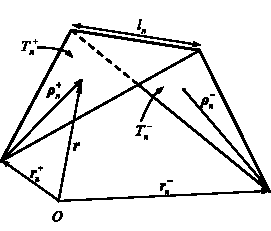
\includegraphics{pica.pdf}
	\caption{RWG 基函数几何参数示意图}
	\label{pica}
\end{figure}
由于时域混合场积分方程是时域电场积分方程与时域磁场积分方程的线性组合,因此时域混合场积分方程时间步进算法的阻抗矩阵特征与时域电场积分方程时间步进算法的阻抗矩阵特征相同。
\begin{equation}
\label{latent_binary_variable}
\mathbf{r}_{i,j}=
\begin{cases}
1,f(\mathbf{x}^{i};\mathbf{w})\cdot f(\mathbf{x}^{j};\mathbf{w})\geq u(\lambda),\\
0,f(\mathbf{x}^{i};\mathbf{w})\cdot f(\mathbf{x}^{j};\mathbf{w})< l(\lambda), 1\leq i,j\leq n.\\
f(\mathbf{x}^{i};\mathbf{w})\cdot f(\mathbf{x}^{j};\mathbf{w}),\text{otherwise},
\end{cases}
\end{equation}

时域积分方程时间步进算法的阻抗元素直接影响算法的后时稳定性,因此阻抗元素的计算是算法的关键之一,采用精度高效的方法计算时域阻抗元素是时域积分方程时间步进算法研究的重点之一。


\subsection{时间基函数}

\subsubsection{时域方法特有的展开函数}

\subsubsection{频域方法特有的展开函数}

\section{入射波}

如图\ref{picb}和图\ref{picc}所示分别给出了参数$E_0=\hat{x}$,$a_n=-\hat{z}$,$f_0=250MHz$,$f_w=50MHz$,$t_w=4.2\sigma$时,调制高斯脉冲的时域与频域归一化波形图。

\begin{figure}[h]
	\subfigure[]{
		\label{picb}
		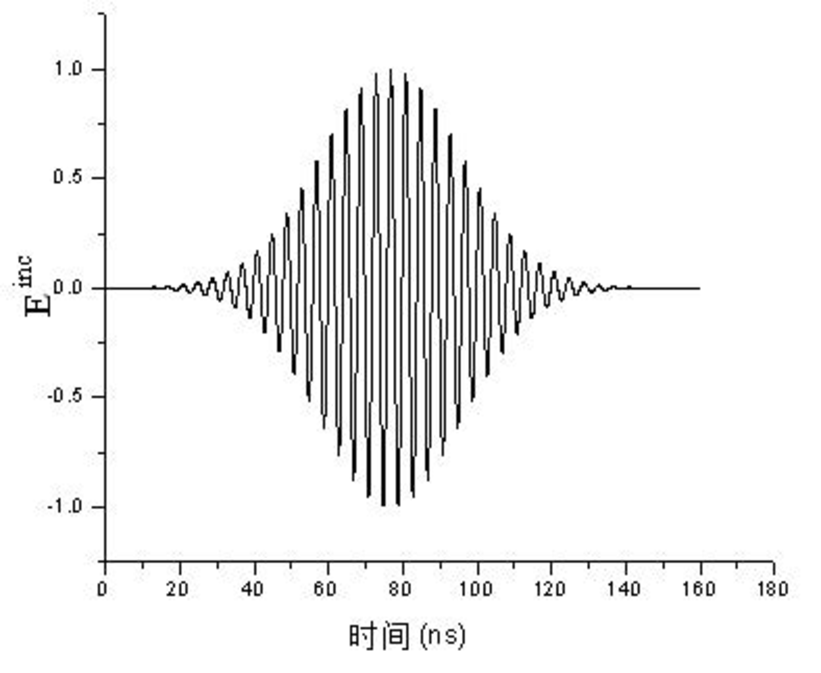
\includegraphics[width=7.3cm]{picb.pdf}}
	\subfigure[]{
		\label{picc}
		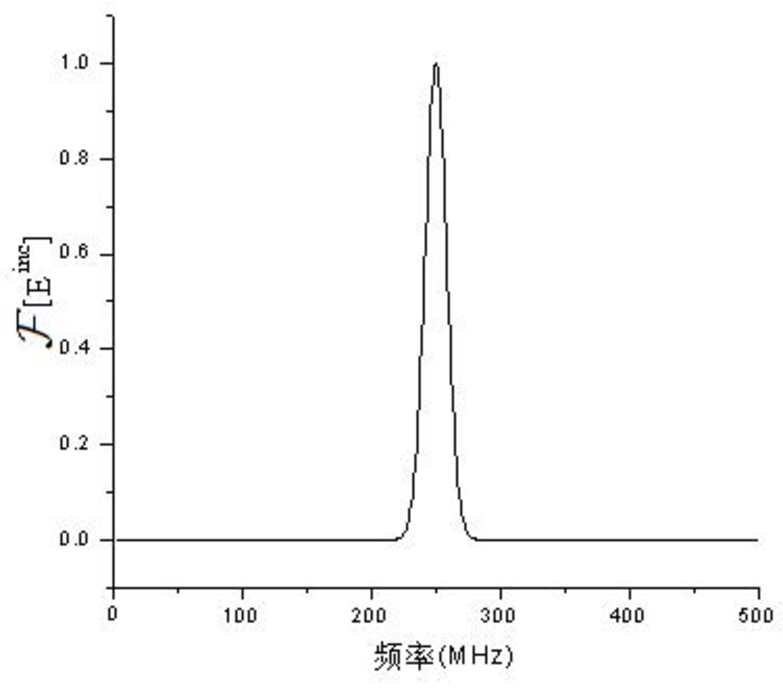
\includegraphics[width=6.41cm]{picc.pdf}}
	\caption{调制高斯脉冲时域与频率波形,时域阻抗元素的存储技术也是时间步进算法并行化的关键技术之一,采用合适的阻抗元素存储方式可以很大的提高并行时间步进算法的计算效率。}
	\label{fig1}
\end{figure}
时域阻抗元素的存储技术\citing{xiao2012yi}也是时间步进算法并行化的关键技术之一,采用合适的阻抗元素存储方式可以很大的提高并行时间步进算法的计算效率。

时域积分方程时间步进算法的阻抗元素直接影响算法的后时稳定性,因此阻抗元素的计算是算法的关键之一,采用精度高效的方法计算时域阻抗元素是时域积分方程时间步进算法研究的重点之一。

\section{时域积分方程时间步进算法阻抗矩阵的存储}
时域阻抗元素的存储技术也是时间步进算法并行化的关键技术之一,采用合适的阻抗元素存储方式可以很大的提高并行时间步进算法的计算效率。

\subsection{时域积分方程时间步进算法产生的阻抗矩阵的特征}
由于时域混合场积分方程是时域电场积分方程与时域磁场积分方程的线性组合,因此时域混合场积分方程时间步进算法的阻抗矩阵特征与时域电场积分方程时间步进算法的阻抗矩阵特征相同。

\subsection{数值算例与分析}

如图3-1(a)所示给出了时间步长选取为0.5ns时采用三种不同存储方式计算的平板中心处 方向的感应电流值与IDFT方法计算结果的比较。如图3-1(b)所示给出了存储方式为基权函数压缩存储方式,时间步长分别取时平板中心处 方向的感应电流计算结果,从图中可以看出不同时间步长的计算结果基本相同。

\begin{algorithm}[H]
	\KwData{this text}
	\KwResult{how to write algorithm with \LaTeX2e }
	initialization\;
	\While{not at end of this document}{
		read current\;
		\eIf{understand}{
			go to next section\;
			current section becomes this one\;
		}{
		go back to the beginning of current section\;
	}
}
\caption{How to wirte an algorithm.}
\end{algorithm}

由于时域混合场积分方程是时域电场积分方程与时域磁场积分方程的线性组合,因此时域混合场积分方程时间步进算法的阻抗矩阵特征与时域电场积分方程时间步进算法的阻抗矩阵特征相同。

\section{时域积分方程时间步进算法矩阵方程的求解}

\section{本章小结}
本章首先研究了时域积分方程时间步进算法的阻抗元素精确计算技术,分别采用DUFFY变换法与卷积积分精度计算法计算时域阻抗元素,通过算例验证了计算方法的高精度。

\end{document}